\section{Note about quad tree sampling}

To speed up the animations, I ported an open-source implementation of quadtree sampling from JavaScript to C++. It works by sorting all of the particles into a structured index (characterized by hierarchical branching of squares within squares). When checking if one of the particles intersects with the macrophage's circle, only those local to the macrophage are checked. Locality is determined and identified by the position in the quadtree. Below, there is a figure in which the local regions of the macrophage are shown in pink. Only the green dots in those squares are checked for collisions. The entire tree index needs to be recreated every frame, but despite this, the speed increase is worth it, especially in the case shown in the image on the right.




\begin{figure}[H]
    \centering
    % First row of two figures
    \begin{subfigure}{0.48\textwidth}
        \centering
        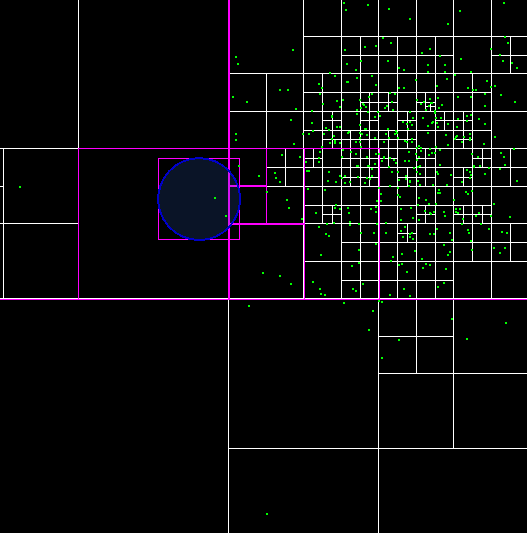
\includegraphics[width=\textwidth]{figures/IMG_ch7/Bursting/QTs/QT1} % Adjust the image path as necessary

        \label{fig:figure1}
    \end{subfigure}
    \hspace{\fill} % Optional: adds space between figures
    \begin{subfigure}{0.48\textwidth}
        \centering
        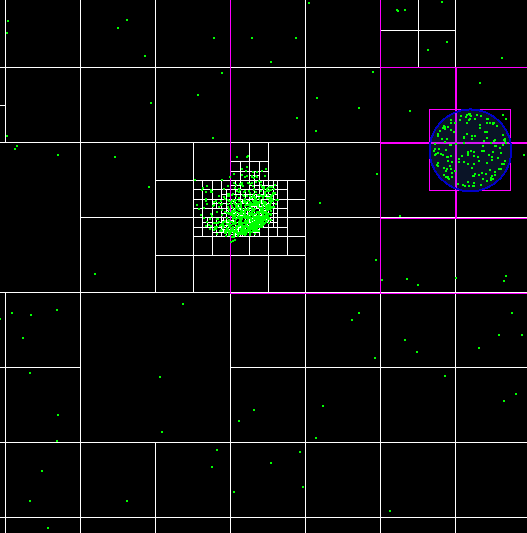
\includegraphics[width=\textwidth]{figures/IMG_ch7/Bursting/QTs/QT2} % Adjust the image path as necessary
      
        \label{fig:figure2}
    \end{subfigure}


    \caption{Visualization of the quadtree sampling used in the particle simulations shown above. Please refer to Wikipedia for more information on this; it's quite a well-worn topic in computer graphics.}
    \label{fig:four_figures}
\end{figure}
